%%%%%%%%%%%%%%%%%%%%%%%%%%%%%%%%%%%%%%%%%
% Jacobs Landscape Poster
% LaTeX Template
% Version 1.1 (14/06/14)
%
% Created by:
% Computational Physics and Biophysics Group, Jacobs University
% https://teamwork.jacobs-university.de:8443/confluence/display/CoPandBiG/LaTeX+Poster
% 
% Further modified by:
% Nathaniel Johnston (nathaniel@njohnston.ca)
%
% This template has been downloaded from:
% http://www.LaTeXTemplates.com
%
% License:
% CC BY-NC-SA 3.0 (http://creativecommons.org/licenses/by-nc-sa/3.0/)
%
%%%%%%%%%%%%%%%%%%%%%%%%%%%%%%%%%%%%%%%%%

%----------------------------------------------------------------------------------------
%	PACKAGES AND OTHER DOCUMENT CONFIGURATIONS
%----------------------------------------------------------------------------------------

\documentclass[final]{beamer}

\usepackage[scale=1.24,orientation=portrait,size=a0]{beamerposter} % Use the beamerposter package for laying out the poster

\usetheme{confposterZ2} % Use the confposter theme supplied with this template

%-----------------------------------------------------------
% Define the column widths and overall poster size
% To set effective sepwid, onecolwid and twocolwid values, first choose how many columns you want and how much separation you want between columns
% In this template, the separation width chosen is 0.024 of the paper width and a 4-column layout
% onecolwid should therefore be (1-(# of columns+1)*sepwid)/# of columns e.g. (1-(4+1)*0.024)/4 = 0.22
% Set twocolwid to be (2*onecolwid)+sepwid = 0.464
% Set threecolwid to be (3*onecolwid)+2*sepwid = 0.708

\newlength{\sepwid}
\newlength{\onecolwid}
%\newlength{\twocolwid}
%\newlength{\threecolwid}
\setlength{\paperwidth}{33.1in} % A0 width: 46.8in 118.8
\setlength{\paperheight}{46in} % A0 height: 33.1in 84.074cm
\setlength{\sepwid}{0.022\paperwidth} % Separation width (white space) between columns
\setlength{\onecolwid}{0.464\paperwidth} % Width of one column 0.464
%\setlength{\twocolwid}{0.8\paperwidth} % Width of two columns 0.928
%\setlength{\threecolwid}{0.708\paperwidth} % Width of three columns
\setlength{\topmargin}{-1.5in} % Reduce the top margin size
%-----------------------------------------------------------

\usepackage{graphicx}  % Required for including images
\usepackage[tight]{subfigure}
\renewcommand*{\thesubfigure}{}

\usepackage{booktabs} % Top and bottom rules for tables
\usepackage{bm}

%----------------------------------------------------------------------------------------
%	TITLE SECTION 
%----------------------------------------------------------------------------------------

\title{A Bandit Framework for Optimal Selection of Reinforcement Learning Agents} % Poster title

%\newcommand*\samethanks[1][\value{footnote}]{\footnotemark[#1]}

\author{A. Merentitis\textsuperscript{1(*)} \and K. Rasul\textsuperscript{2}, \and R. Vollgraf\textsuperscript{2}, \and A. S. Sheikh\textsuperscript{2}, \and U. Bergmann\textsuperscript{2}
}

\institute{OLX Berlin Hub, Zalando Research} % Institution(s)

%----------------------------------------------------------------------------------------

\begin{document}

\addtobeamertemplate{headline}{} 
{
\begin{tikzpicture}[remember picture,overlay] 
\node [shift={(-9.8 cm,-5.5cm)}] at (current page.north east) {
\includegraphics[height=4.4cm]{common_images/ZR}}; 
\end{tikzpicture} 
}

\addtobeamertemplate{headline}{} 
{
\begin{tikzpicture}[remember picture,overlay] 
\node [shift={(-65 cm,-5.5cm)}] at (current page.north east) {
\includegraphics[height=3.6cm]{common_images/OLX_Logo_Core_Charcoal_RGB_HR}}; 
\end{tikzpicture} 
}

\addtobeamertemplate{headline}{} 
{
\begin{tikzpicture}[remember picture,overlay] 
\node [shift={(-78 cm,-5.5cm)}] at (current page.north east) {
\includegraphics[height=3.6cm]{common_images/nips_small}}; 
\end{tikzpicture} 
}


\addtobeamertemplate{block end}{}{\vspace*{1.2ex}} % White space under blocks
\addtobeamertemplate{block alerted end}{}{\vspace*{2ex}} % White space under highlighted (alert) blocks

\setlength{\belowcaptionskip}{2ex} % White space under figures
\setlength\belowdisplayshortskip{2ex} % White space under equations


\vspace*{-2.5cm}

\begin{frame}[t] % The whole poster is enclosed in one beamer frame

\begin{columns}[t] 

\begin{column}{\sepwid}\end{column} % Empty spacer column

\begin{column}{\onecolwid} % The first column

%----------------------------------------------------------------------------------------
\begin{block}{Motivation}
\begin{itemize}

\item The optimal inductive bias (architecture, hyperparameters, etc.) of a RL agent depends on the application. 
\item We propose a multi-arm bandit with the double objective of maximizing the reward while the agents are learning and selecting the best agent after a small number of learning steps. 
\end{itemize}

\end{block}
\vspace*{-0.5cm}

\begin{block}{Multi-arm bandit framework}

Different types of bandit strategies are possible, from simple $\epsilon$-greedy, to techniques like SoftMax (probability matching bandit), UCB1 (based on the optimism in the face of uncertainty principle) and EXP3 (adversarial bandit). 

\vspace*{0.5cm}

It has been shown in [Yi-Sun-2011] that it is beneficial for agents to take actions that maximize the reduction in uncertainty about the environment dynamics. This can be formalized as taking a sequence of actions $a_t$ that maximize the sum of reductions in entropy. With the history of the agents up until time step $t$ as $\xi_{t} = \{s_1 , a_1 , \dots , s_t \}$, we can write the sum of entropy reductions as:

\begin{equation}
        \sum_{t} \left( H\left(\bold\mathbf{\Theta}| \xi_{t}, a_t \right) - H \left(\bold\mathbf{\Theta} | S_{t+1}, \xi_{t}, a_t \right) \right). \label{eq:1}
\end{equation}

As indicated in [Houthooft-2016], according to information theory, the individual terms express the mutual information between the next state distribution $S_{t+1}$ 
and the model parameter distribution $\bold\mathbf{\Theta}$, namely $I(S_{t+1}; \bold\mathbf{\Theta}|\xi_{t},a_{t})$. This mutual information can be written as:

\begin{equation}
       I \left (S_{t+1};\bold\mathbf{\Theta}|\xi_{t},a_{t} \right) = \mathbb{E}_{s_{t+1} \sim P \left(\cdot|\xi_{t},a_{t} \right)} [D_{KL}[p \left(\theta|\xi_{t},a_t,s_{t+1}\right) || p \left(\theta|\xi_{t} \right)]], \label{eq:2}
\end{equation}

\vspace*{0.5cm}

The KL divergence term is expressing the difference between the new and the old beliefs of the agent regarding the environment dynamics, and the expectation is with respect. Under these assumptions the above formulation can also be interpreted as information gain [Houthooft-2016] according to the Variational Information Maximizing Exploration (VIME) exploration strategy.


\end{block}
\vspace*{-0.5cm}
\begin{block}{Calculating the information gain}

Formally, since calculating the posterior $p(\theta|D)$ for a dataset $D$ is not feasible, we follow VIME and approximate it through an alternative distribution $q(\theta;\phi)$, parametrized by $\phi$. In this setting we seek to minimize $D_{KL}$ through maximization of the variational lower bound $L[q(\theta ; \phi),D]$. The latter is formulated as:

\begin{equation}
        L[q(\theta ; \phi),D] =  \mathbb{E}_{\theta \sim q(\cdot ; \phi)} [\log p(D|\theta)] - D_{KL}[q(\theta ; \phi) || p(\theta)]. \label{eq:3}
\end{equation}

%Then we can derive the information gain terms as:
The information gain term can then can be expressed as:


\begin{equation}
       I(S_{t+1}; \bold\mathbf{\Theta}|\xi_{t},a_{t}) = D_{KL} [q(\theta ; \phi_{t+1}) || q(\theta ; \phi)], \label{eq:4}
\end{equation}
where $\phi_{t+1}$ represents the updated and $\phi_{t}$ the old parameters of the agent's belief regarding the environment dynamics.

\end{block}

\setbeamercolor{block alerted title}{fg=black,bg=Zalando} % Change the alert block title colors
\setbeamercolor{block alerted body}{fg=black,bg=white} % Change the alert block body colors

\begin{block}{Relation between information gain and true environment rewards}

\begin{figure}[h!]
   \begin{tabular}{ll}
    	 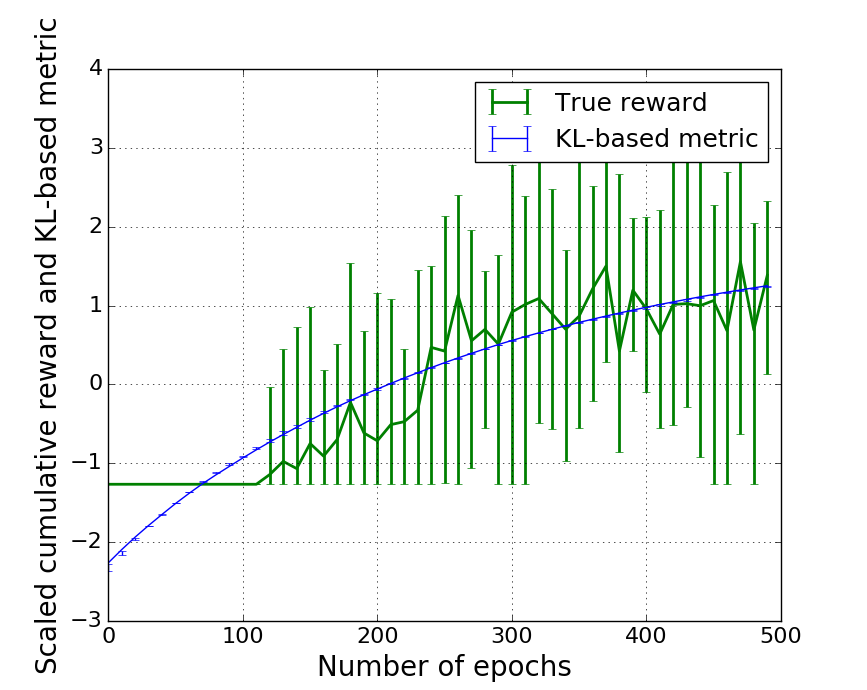
\includegraphics[width=0.5\columnwidth]{misc/mountaincar_correlation.png} &
		 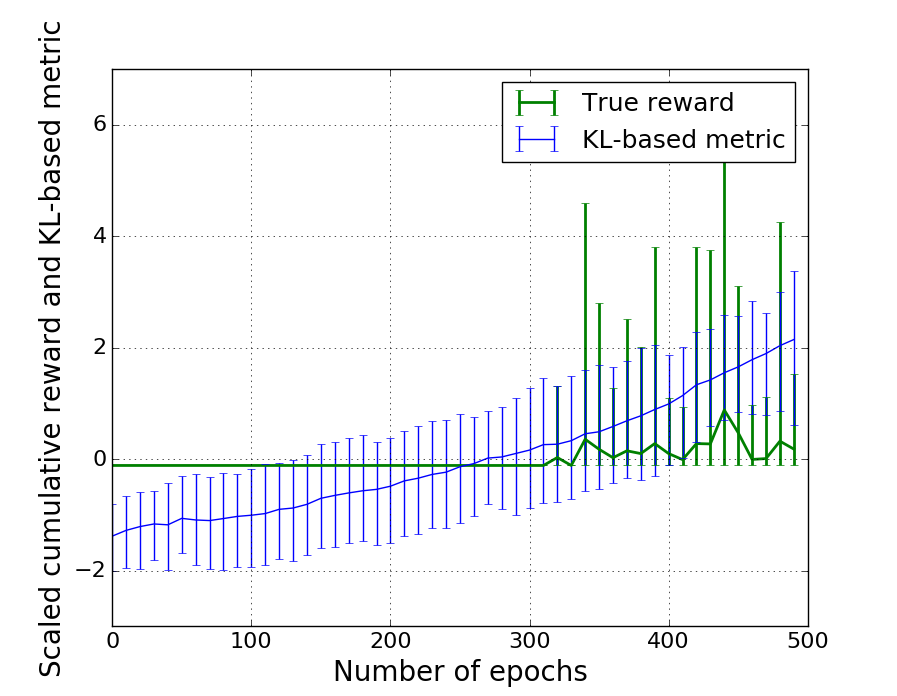
\includegraphics[width=0.5\columnwidth]{misc/mountaincar_correlation_badagent.png} \\
	 \end{tabular}
   \vspace{-0.4cm}\caption{\em Correlation between environment and information gain rewards for a good (left) and a suboptimal agent (right) for Mountain Car environment.}
\label{fig:correlation_check}
\end{figure}

\end{block}

\vspace*{-1.5cm}

\begin{block}{What we gain with surrogate rewards}

\vspace{-0.5\baselineskip}

\begin{itemize}
\item To alleviate the problem of sparse rewards, the reinforcement learning agents are augmented with surrogate rewards. 
\item This helps the bandit framework to select the best agents early, since these rewards are smoother and less sparse than the environment reward. 
\end{itemize}

\end{block}

\vspace*{-0.5cm}

\begin{footnotesize}
\begin{itemize}
\item \textit{1: OLX Berlin Hub}
\item \textit{2: Zalando Research}
\end{itemize}

(*) Most of this work was done while the author worked at Zalando Research

\end{footnotesize}


\end{column} % End of the first column

\begin{column}{\sepwid}\end{column} % Empty spacer column

%\begin{column}{\sepwid}\end{column} % Empty spacer column

\begin{column}{\onecolwid} % The second column

%----------------------------------------------------------------------------------------

\begin{block}{Cumulative surrogate and true environment rewards}

\begin{figure}[h!]

Cumulative surrogate reward for Cartpole and Mountain Car envs.
{%
\begin{tabular}{ll}
    	 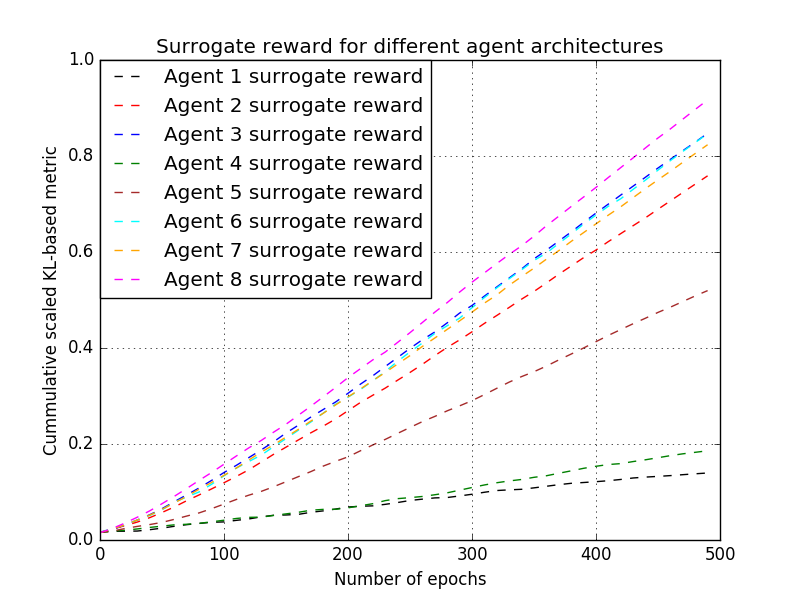
\includegraphics[width=0.45\columnwidth]{misc/cart_surrogate.png} &
		 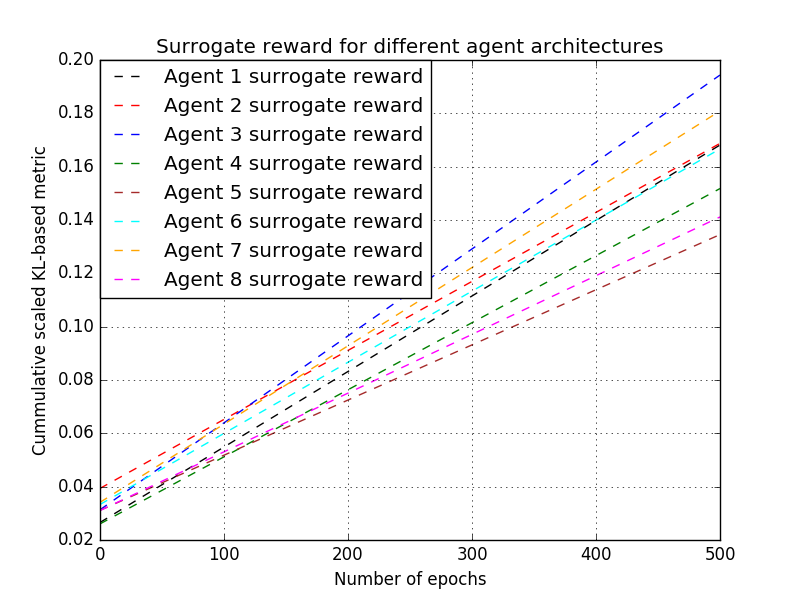
\includegraphics[width=0.45\columnwidth]{misc/mc_surrogate.png} \\
	 \end{tabular}
}

Cumulative true reward for Cartpole and Mountain Car envs.
{%
\begin{tabular}{ll}
    	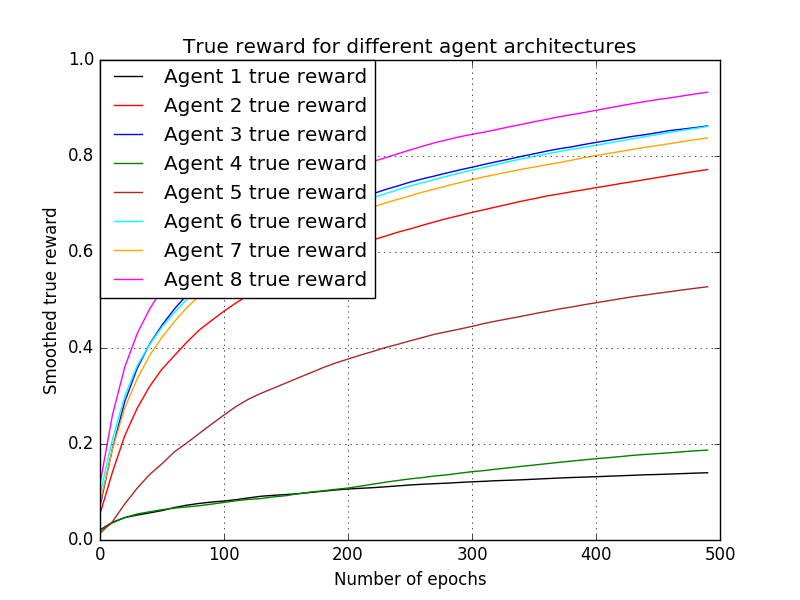
\includegraphics[width=0.45\columnwidth]{misc/cart_true.png} &
		 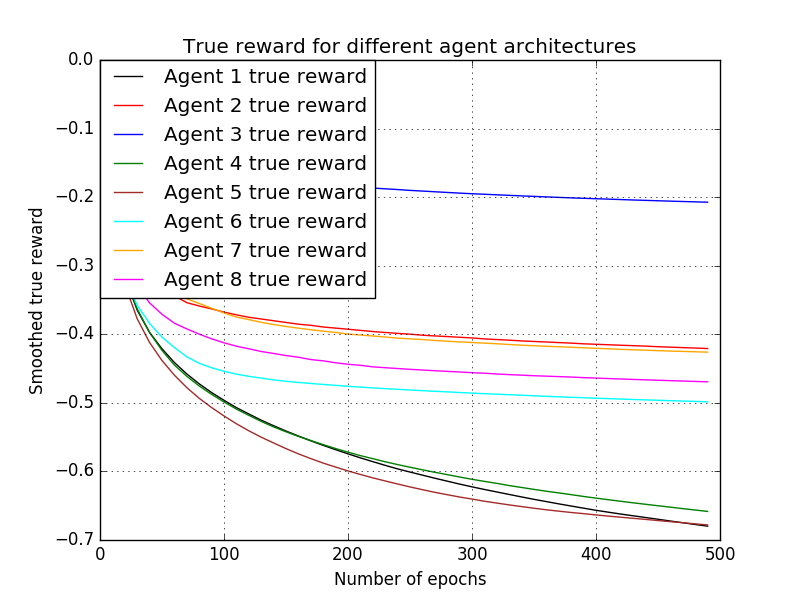
\includegraphics[width=0.45\columnwidth]{misc/mc_true.png} \\
	 \end{tabular}
}

\caption{Comparison of the scaled cumulative surrogate and true rewards for the Cartpole and Mountain Car environments for different reinforcement learning agents. The relative order of the agents is similar between the first and second rows, indicating that the surrogate reward can be used to augment the true reward, especially early on when the latter is sparse and noisy.}
\label{fig:cart_mc_rewards}
\end{figure}

\end{block}

\vspace*{-1.5cm}

\begin{block}{Frequency of selections of the different agents}

\vspace*{-1.5cm}

\begin{figure}[h!]
   \begin{tabular}{ll}
     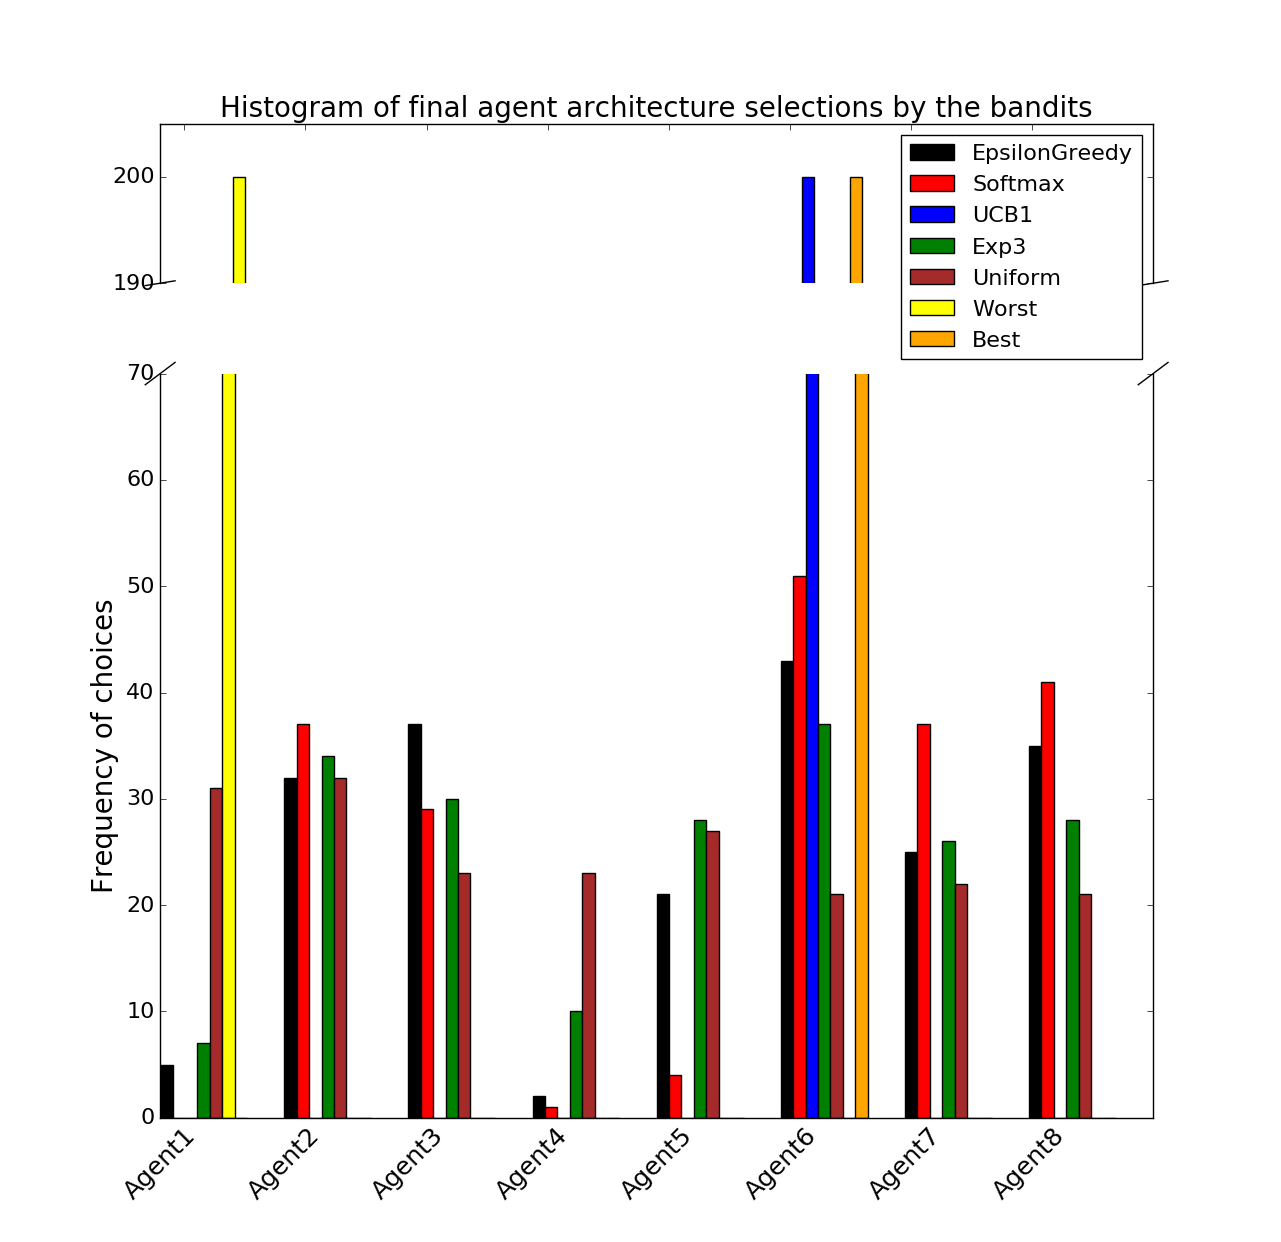
\includegraphics[width=0.5\columnwidth]{misc/lunar_bar.png} &
	 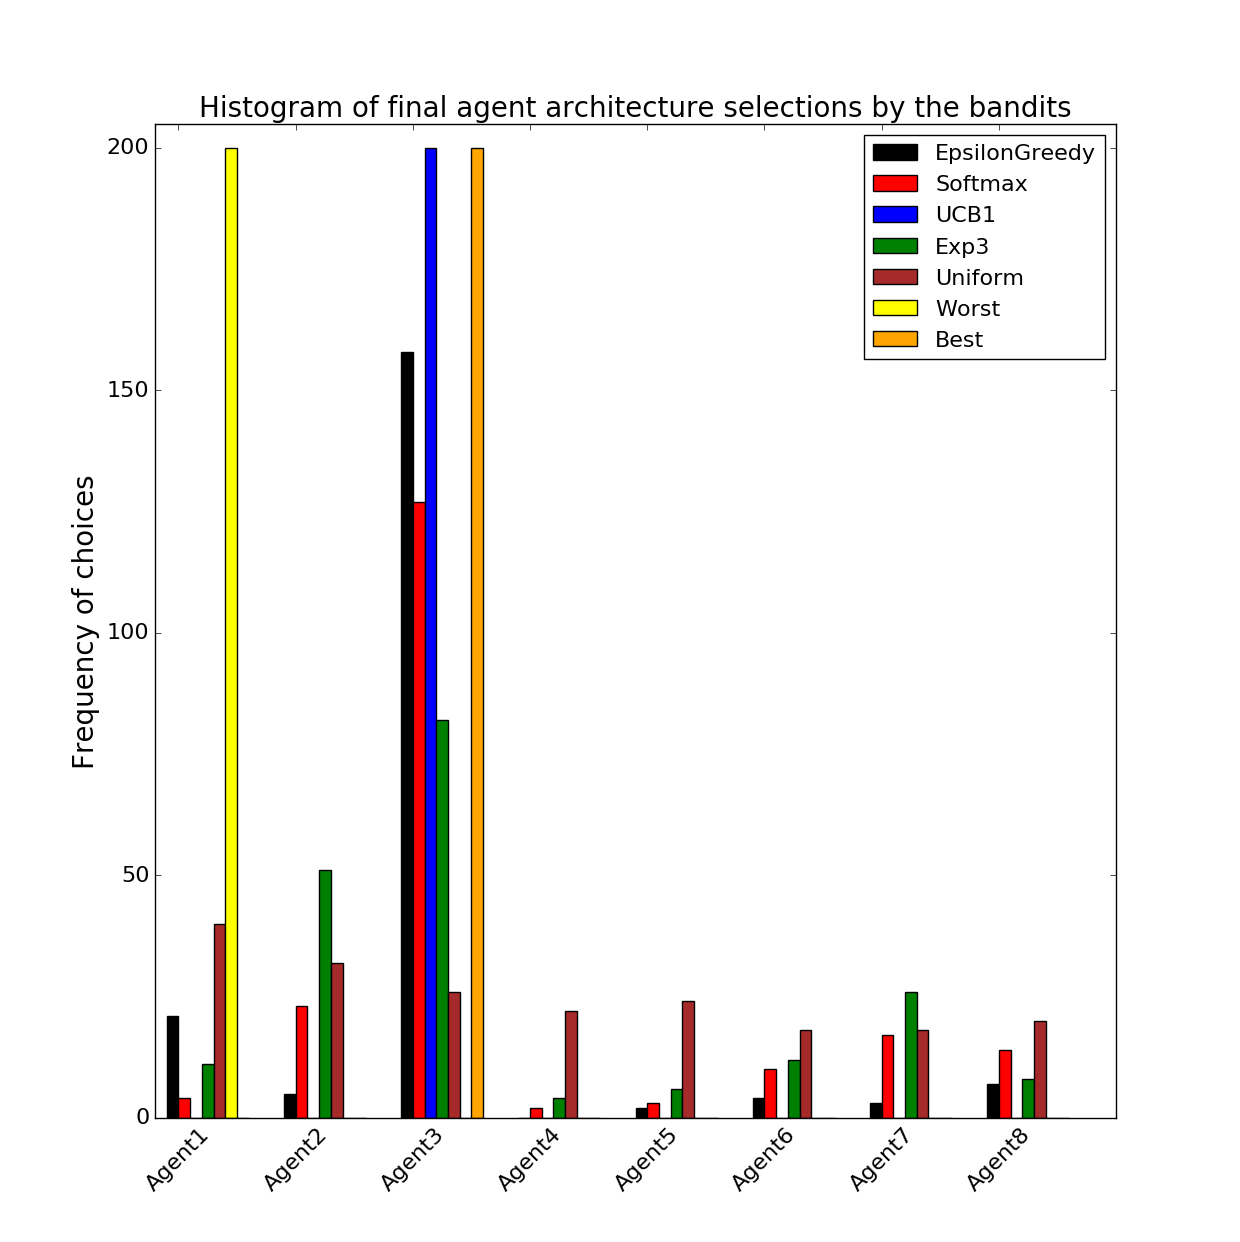
\includegraphics[width=0.5\columnwidth]{misc/mc_bar2.png} \\
	 \end{tabular}
   \caption{\em Frequency of selections of the different agents for Lunar Lander (left) and Mountain Car (right) at the end of training for the different bandit algorithms. The UCB
   algorithm matches the oracle (Best) in selecting the best agent after training is complete.}
\label{fig:lunar_mc_bar}
\end{figure}

\end{block}

\vspace*{-1.5cm}

\begin{block}{Score for DQN, Gorila, pro human gamer, and the agent selected from the bandit}

  \centering
  \begin{tabular}{|p{5.5cm}|p{6.5cm}|l|p{4.5cm}|p{7.5cm}|}
  \hline
  Games & DQN Score & Gorila Score & Human Pro Score & Best Agent Score\\
  \hline
    Atlantis            & 85641 $\pm$ 17600 & 100069.16 & 29028 & 217810 $\pm$ 7256.4 \\
    Kung-Fu             & 23270 $\pm$  5955 & 27543.33  & 22736 & 29860  $\pm$  6793.1 \\
    Ms. Pacman          &  2311 $\pm$   525 & 3233.50   & 15693 & 5708.0 $\pm$  860.1 \\
    Seaquest            &  5286 $\pm$  1310 & 13169.06  & 20182 & 17214  $\pm$ 2411.5 \\
    Sp. Invaders        &  1976 $\pm$   893 & 1883.41   &  1652 & 3697.5 $\pm$ 2876.1 \\
    Zaxxon              &  4977 $\pm$  1235 & 7129.33   &  9173 & 30610  $\pm$ 8169.0 \\
  \hline  
  \end{tabular}
  \label{tab:1}

\end{block}

\begin{block}{Conclusions}

\begin{itemize}
\item Introduced a bandit framework that offers a principled way of selecting between different RL agent architectures. 
\item Maximizing rewards during the learning process.
\item Reliably select the best agent (in future expected rewards). 
\item Composite surrogate reward captures the certainty of the agents regarding the environment dynamics, for a given amount of environment interactions.
\item Experimental results show that the bandit outperforms both a single non-optimal agent and uniform alternation between the agents.
\end{itemize}

\end{block}

%\vspace*{-1.5cm}

\begin{footnotesize}
\begin{itemize}
\item \textit{"Planning to Be Surprised: Optimal Bayesian Exploration in Dynamic Environments", Yi-Sun et al. 2011}
\item \textit{"Curiosity-driven Exploration in Deep Reinforcement Learning via Bayesian
Neural Networks", Houthooft et al. 2016}
\end{itemize}

\end{footnotesize}

\end{column} % End of the second column

\end{columns} % End of all the columns in the poster

\end{frame} % End of the enclosing frame

\end{document}
